\section{Evaluation}
We evaluated our algorithms using the following real life traces: (1) CAIDA'16: CAIDA Internet Traces from ``Equinix-Chicago'' in 2016~\cite{CAIDA2016}, (2) CAIDA'18: CAIDA Internet Traces from ``Equinix-NewYork'' in 2018~\cite{CAIDA2018}. We considered IP source hierarchies in a single bit granularities, such hierarchies were also used in~\cite{ben2017constant, SpaceSaving}, and considered the unweighted frequencies of items (i.e., the number of packets). Each data point is the average of 10 runs, where each run started from a randomly selected point in the given trace.

We use the \textit{Recall} and \textit{Precision} metrics proposed in ~\cite{ffMetrics} to evaluate the performance of the suggested algorithms. In order to compute these metrics, we calculated the true set of HH and HHH using a space intensive algorithm that allocates a counter per flow for exact measurements.
Recall is the number of true HHHs detected by the algorithm divided by the number of true HHHs. This metric is equivalent to the Detection Rate of the algorithm, i.e., what is the percentage of HHHs the algorithm detects.
Precision is the number of true HHHs detected by the algorithm divided by the number of reported suspect HHH. This metric complements the false positive rate of the algorithm and tries to grasp how many of the suspect HHHs the algorithm was mistaken.

We denote our proposed algorithms with ``SS" for \simpleAlgo, ``MS" for \multipleAlgo, ``HTF" for \ref{algo:htf} and ``SA" for \ref{algo:sa}. Furthermore, we use ``RHHH" to denote the algorithm proposed in~\cite{ben2017constant} and ``MST" to denote the algorithm proposed in~\cite{SpaceSaving}. These algorithms solve an approximate version of the problem with an accuracy parameter $\epsilon$, when comparing with them we expand the set of true HHH by a slack of $\epsilon T$.

\begin{figure}
    \centering
    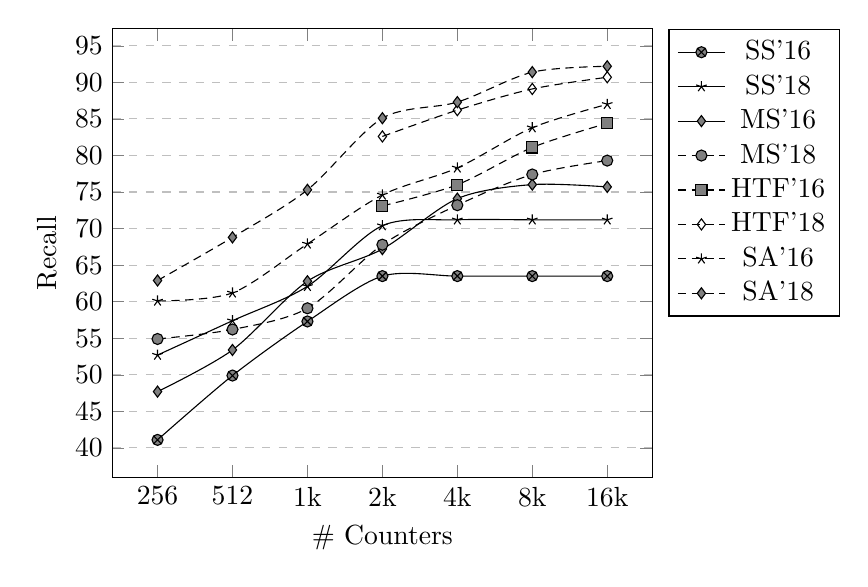
\begin{tikzpicture}
        \begin{axis}[
        xlabel={\# Counters},
        ylabel={Recall},
        xtick=data,
        xticklabels={256, 512, 1k, 2k, 4k, 8k, 16k},
        ytick={0,5,10,15,20,25,30,35,40,45,50,55,60,65,70,75,80,85,90,95,100},
        % legend pos=south east,
        % legend columns=2,
        ymajorgrids=true,
        grid style=dashed,
        legend style ={ at={(1.03,1)}, 
        anchor=north west, draw=black, 
        fill=white,align=left},
        cycle list name=black white,
        smooth
        ]
            \addplot
            coordinates {
                (1,41.1)(2,49.9)(3,57.3)(4,63.5)(5,63.5)(6,63.5)(7,63.5)
            };
            \addlegendentry{SS'16};
            \addplot
            coordinates {
                (1,52.7)(2,57.4)(3,62.1)(4,70.4)(5,71.2)(6,71.2)(7,71.2)
            };
            \addlegendentry{SS'18};
            \addplot
            coordinates {
                (1,47.7)(2,53.4)(3,62.8)(4,67.2)(5,74.1)(6,76.02)(7,75.7)
            };
            \addlegendentry{MS'16};
            \addplot
            coordinates {
                (1,54.9)(2,56.2)(3,59.1)(4,67.8)(5,73.2)(6,77.4)(7,79.3)
            };
            \addlegendentry{MS'18};
            \addplot
            coordinates {
                (4,73.1)(5,76.0)(6,81.1)(7,84.4)
            };
            \addlegendentry{HTF'16};
            \addplot+[black, mark=diamond]
            coordinates {
                (4,82.6)(5,86.2)(6,89.1)(7,90.7)
            };
            \addlegendentry{HTF'18};
            \addplot
            coordinates {
                (1,60.1)(2,61.2)(3,67.9)(4,74.6)(5,78.3)(6,83.8)(7,87.0)
            };
            \addlegendentry{SA'16};
            \addplot
            coordinates {
              (1,62.9)(2,68.8)(3,75.3)(4,85.1)(5,87.3)(6,91.4)(7,92.2)
            };
            \addlegendentry{SA'18};
        \end{axis}
    \end{tikzpicture}
    \caption{The Recall of the algorithms for various number of counters on CAIDA'16 and CAIDA'18 traces.}
    \label{fig:recall}
\end{figure}

Figure~\ref{fig:recall} shows the \textit{Recall} of the various algorithms as a function of the number of available counters. Each line describes a single algorithm and the CAIDA trace, the runs are on random parts of the trace of $2^{25}$ packets (about one minute of traffic) with threshold $\phi=0.001$. It is worthy to note that the performance on CAIDA'18 trace is usually better than those of CAIDA'16 trace, this is since in CAIDA'16 trace the heaviest flows are not as stable as in CAIDA'18. Also, note that the number of HH in these traces at a given level of the hierarchy is at most 200. This explains the overall poor performance when using fewer counters than 512.

When considering the Recall of ~\simpleAlgo and ~\multipleAlgo algorithms, one can notice an improvement as the number of counters increases up to a point where adding more counters does not help anymore. This limitation is explained by the lack of a retracting mechanism in these algorithms, thus missing a portion of the HHH that starts late in the monitoring interval and more specifically after the first round.

The ~\ref{algo:htf} Algorithm can not run properly for a very low number of counters, that is up to $1k$ counters. That is due to the fact that sometimes the attempt to retract the frontier does not free enough counters to perform full refinement of the interesting flowsets. Thus, we did not report the results for the number of counters where at least one run of the algorithm did not finish due to this reason. For a higher number of counters (starting from $2k$) the algorithm manages to breach the observed limitation at ~\simpleAlgo and ~\multipleAlgo algorithms due to its retracting mechanism.

The main advantage of ~\ref{algo:sa} algorithm compared to ~\ref{algo:htf} algorithm lies in the ability to deploy it using a smaller number of counters. The difference in the recall of the algorithms is not statistically significant, where both reach around 90\% recall on the CAIDA'18 traces.

\begin{figure}
    \centering
    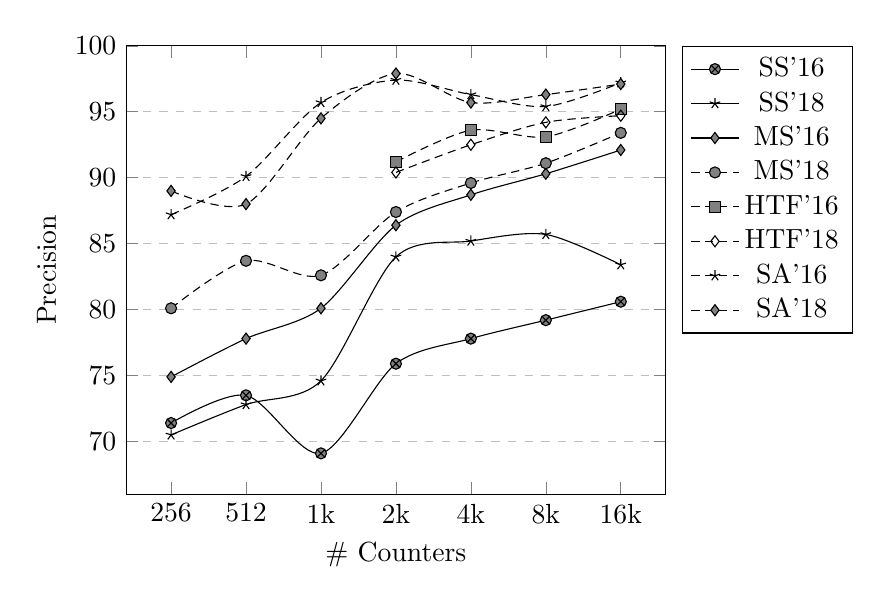
\begin{tikzpicture}
        \begin{axis}[
        xlabel={\# Counters},
        ylabel={Precision},
        xtick=data,
        xticklabels={256, 512, 1k, 2k, 4k, 8k, 16k},
        ytick={0,5,10,15,20,25,30,35,40,45,50,55,60,65,70,75,80,85,90,95,100},
        % legend pos=south east,
        % legend columns=2,
        ymajorgrids=true,
        ymax=100,
        grid style=dashed,
        legend style ={ at={(1.03,1)}, 
        anchor=north west, draw=black, 
        fill=white,align=left},
        cycle list name=black white,
        smooth
        ]
            \addplot
            coordinates {
                (1,71.4)(2,73.5)(3,69.1)(4,75.9)(5,77.8)(6,79.2)(7,80.6)
            };
            \addlegendentry{SS'16};
            \addplot
            coordinates {
                (1,70.5)(2,72.8)(3,74.6)(4,84.0)(5,85.2)(6,85.7)(7,83.4)
            };
            \addlegendentry{SS'18};
            \addplot
            coordinates {
                (1,74.9)(2,77.8)(3,80.1)(4,86.4)(5,88.7)(6,90.3)(7,92.1)
            };
            \addlegendentry{MS'16};
            \addplot
            coordinates {
                (1,80.1)(2,83.7)(3,82.6)(4,87.4)(5,89.6)(6,91.1)(7,93.4)
            };
            \addlegendentry{MS'18};
            \addplot
            coordinates {
                (4,91.2)(5,93.6)(6,93.1)(7,95.2)
            };
            \addlegendentry{HTF'16};
            \addplot+[black, mark=diamond]
            coordinates {
                (4,90.4)(5,92.5)(6,94.2)(7,94.7)
            };
            \addlegendentry{HTF'18};
            \addplot
            coordinates {
                (1,87.2)(2,90.1)(3,95.7)(4,97.4)(5,96.3)(6,95.4)(7,97.2)
            };
            \addlegendentry{SA'16};
            \addplot
            coordinates {
                (1,89.0)(2,88.0)(3,94.5)(4,97.9)(5,95.7)(6,96.3)(7,97.1)
            };
            \addlegendentry{SA'18};
        \end{axis}
    \end{tikzpicture}
    \caption{The Precision of the algorithms for various number of counters on CAIDA'16 and CAIDA'18 traces.}
    \label{fig:precision}
\end{figure}

Figure~\ref{fig:precision} depicts the \textit{Precision} of the various algorithms as a function of the number of available counters in the same settings as Figure~\ref{fig:recall}. More specifically, the figure shows how many flows reported by the algorithm as HHH were actually a true HHH, i.e., how precise was the algorithm in its reports. All of our algorithms tend to report most of their false positives, reported flows that are not HHH, in the higher levels of the hierarchy. Due to the parts of the hierarchy that are not monitored but still see some traffic, however, in lower levels the algorithms have a better estimation of the flow's frequencies and whether they are HHH or not. Furthermore, the higher in the hierarchy the calculation of HHH happens, the more it is prone to errors due to errors in the lower levels.

We note that the difference in precision between the two traces in a given algorithm is not that noticeable. This is explained by the fact that if even in CAIDA'16 the heaviest flows are not consistent compared to CAIDA'18, the algorithms manage to filter out flows that lead to splitting at higher levels but did not remain suspect HH throughout the rounds.

Furthermore, the trend of better performance with more counter we observed in Figure~\ref{fig:recall} is less clear especially in ~\simpleAlgo and ~\multipleAlgo algorithms. That is, sometimes more counters lead to a small decrease in the precision of the algorithms. This might be explained by the fact that with more counters these simple algorithms focus on more unimportant parts down the hierarchy.

The precision of ~\ref{algo:sa} Algorithm reaches more than 95\% for $1k$ counters and even around 97\% for more than that. This means, that given enough counters this algorithm detects around 90\% of the true HHH and reports no more than 3\% non-HHH flows. For the same reasons mentioned before, the results of ~\ref{algo:htf} Algorithm were not reported for counters less than $2k$.

\begin{figure}
    \centering
    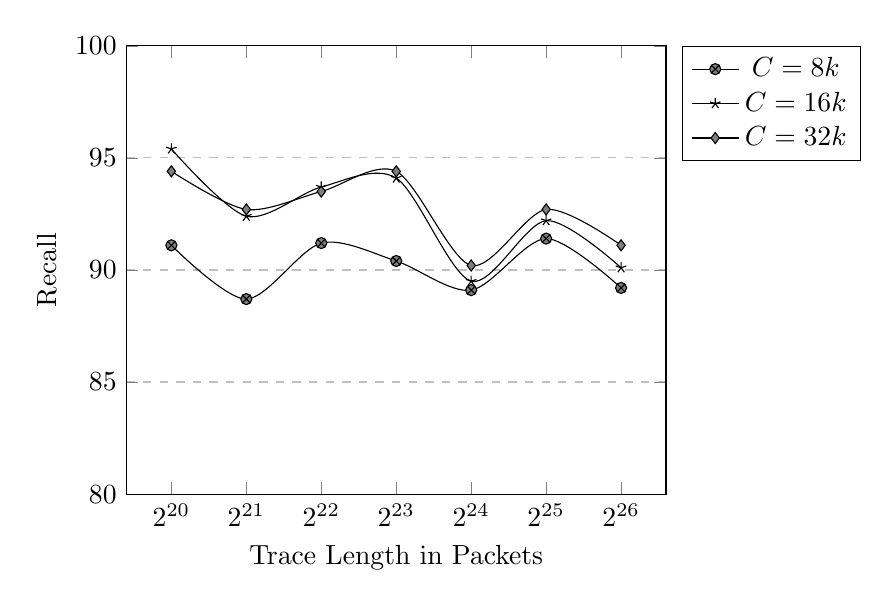
\begin{tikzpicture}
        \begin{axis}[
        xlabel={Trace Length in Packets},
        ylabel={Recall},
        xtick=data,
        xticklabels={$2^{20}$, $2^{21}$, $2^{22}$, $2^{23}$, $2^{24}$, $2^{25}$, $2^{26}$},
        ytick={0,5,10,15,20,25,30,35,40,45,50,55,60,65,70,75,80,85,90,95,100},
        % legend pos=south east,
        % legend columns=2,
        ymajorgrids=true,
        ymax=100,
        ymin=80,
        grid style=dashed,
        legend style ={ at={(1.03,1)}, 
        anchor=north west, draw=black, 
        fill=white,align=left},
        cycle list name=black white,
        smooth
        ]
            \addplot
            coordinates {
                (1,91.1)(2,88.7)(3,91.2)(4,90.4)(5,89.1)(6,91.4)(7,89.2)
            };
            \addlegendentry{$C=8k$};
            \addplot
            coordinates {
                (1,95.4)(2,92.4)(3,93.7)(4,94.1)(5,89.5)(6,92.2)(7,90.1)
            };
            \addlegendentry{$C=16k$};
            \pgfplotsset{cycle list shift=2}
            \addplot
            coordinates {
                (1,94.4)(2,92.7)(3,93.5)(4,94.4)(5,90.2)(6,92.7)(7,91.1)
            };
            \addlegendentry{$C=32k$};
        \end{axis}
    \end{tikzpicture}
    \caption[Recall of ~\ref{algo:sa} Algorithm as function of the trace length]{The recall of~\ref{algo:sa} Algorithm for various length of trace on CAIDA'18.}
    \label{fig:trace_length}
\end{figure}

Figure~\ref{fig:trace_length} depicts the recall of ~\ref{algo:sa} Algorithm (under the same settings) as a function of the trace length (number of packets processed) for a given number of counters. It easy to see that the algorithm does not require any convergence period in order to achieve high recall. Furthermore, there is no consistent trend in the recall of the algorithm as a function of the trace length, besides slight variations that can be explained as fluctuations in the different parts of the trace.

\begin{figure}
    \centering
    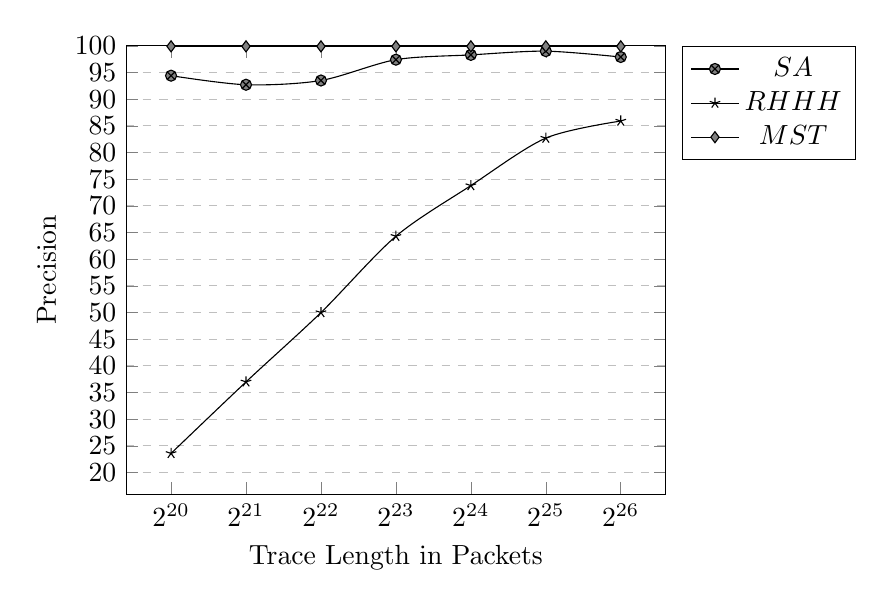
\begin{tikzpicture}
        \begin{axis}[
        xlabel={Trace Length in Packets},
        ylabel={Precision},
        xtick=data,
        xticklabels={$2^{20}$, $2^{21}$, $2^{22}$, $2^{23}$, $2^{24}$, $2^{25}$, $2^{26}$},
        ytick={0,5,10,15,20,25,30,35,40,45,50,55,60,65,70,75,80,85,90,95,100},
        % legend pos=south east,
        % legend columns=2,
        ymajorgrids=true,
        ymax=100,
        grid style=dashed,
        legend style ={ at={(1.03,1)}, 
        anchor=north west, draw=black, 
        fill=white,align=left},
        cycle list name=black white,
        smooth
        ]
            \addplot
            coordinates {
                (1,94.4)(2,92.7)(3,93.5)(4,97.4)(5,98.3)(6,99.0)(7,97.9)
            };
            \addlegendentry{$SA$};
            \addplot
            coordinates {
                (1,23.6)(2,37.0)(3,50.0)(4,64.3)(5,73.8)(6,82.7)(7,85.9)
            };
            \addlegendentry{$RHHH$};
            \pgfplotsset{cycle list shift=2}
            \addplot
            coordinates {
                (1,99.9)(2,99.9)(3,99.9)(4,99.9)(5,99.9)(6,99.9)(7,99.9)
            };
            \addlegendentry{$MST$};
        \end{axis}
    \end{tikzpicture}
    \caption{The precision of ~\ref{algo:sa} Algorithm compared to ``MST" and ``RHHH" on CAIDA'16 trace, for $\phi=0.01, \epsilon=0.001, C=\frac{H}{\epsilon}=\frac{32}{0.001}=32k$ on single bit IP source hierarchy for various lengths the trace.}
    \label{fig:trace_length_precision}
\end{figure}




Figure~\ref{fig:trace_length_precision} depicts the precision of the ~\ref{algo:sa} algorithm as function of the trace length (number of packets processed) compared to ``MST" and ``RHHH". As expected, ``RHHH" suffers from a convergence interval, only then it starts to keep its probabilistic guarantees of low false positive. ``MST", which requires $O(H)$ update time per-packet, achieves almost perfect precision (no false positive) as guaranteed by $\epsilon$. Our ~\ref{algo:sa} algorithm achieves a high precision rate averaged around 95\% regardless of the trace's length while holding $O(1)$ per-packet update time. The algorithms converge similarly on CAIDA`18 traces.
